\documentclass[11pt, a4paper, twocolumn]{article}

%%%%%%%%%%%%%%%%%
% Configuration %
%%%%%%%%%%%%%%%%%
\usepackage{allrunes}
\usepackage{amsmath}
% If magyar is wanted
%\usepackage[magyar]{babel}

\usepackage[T1]{fontenc}
\usepackage[utf8]{inputenc}
\usepackage{fixltx2e}
\usepackage{multirow}
\usepackage{url}
\usepackage{amsfonts}
\usepackage{amsthm}
\usepackage{amssymb}
\usepackage{xcolor}

\newcommand{\abstractText}{\noindent
  Abstract goes here.
}

% Here you can configure the layout
\usepackage{geometry}
\geometry{top=1cm, bottom=1cm, left=1.25cm,right=1.25cm, includehead, includefoot}
\setlength{\columnsep}{7mm} % Column separation width

\usepackage{graphicx}

%\usepackage{gensymb}
\usepackage{float}

% For bra-ket notation
\usepackage{braket}

% To have a good appendix
\usepackage[toc,page]{appendix}

\usepackage{abstract}
\renewcommand{\abstractnamefont}{\normalfont\bfseries}
\renewcommand{\abstracttextfont}{\normalfont\small\itshape}
\usepackage{lipsum}

%%%%%%%%%%%%%%%%%%%
% Custom commands %
%%%%%%%%%%%%%%%%%%%
\newcommand{\bb}[1]{\mathbf{#1}}
\newcommand{\dd}{\mathrm{d}}


% Hyperref should be generally the last package to load
% Any configuration that should be done before the end of the preamble:
\usepackage{hyperref}
\hypersetup{colorlinks=true, urlcolor=blue, linkcolor=blue, citecolor=blue}

\title{Numerical simulation of quantum transport phenomena}

\author{Nagy Dániel}

\begin{document}

%%%%%%%%%%%%
% Abstract %
%%%%%%%%%%%%

\twocolumn[
  \begin{@twocolumnfalse}
    \maketitle
    \begin{abstract}
      In recent years electronic transport properties of a variety of low dimensional electron systems,
    such as carbon based novel materials like carbon nanotubes or graphene, boron nitride, dichalcogenides, 
    a selection of intriguing molecules and the surface states of topological insulators has captured the imagination of the 
    solid-state community. These systems have several interesting properties that make them not only interesting for theoretical 
    investigations but could also lead to revolutionary applications from wearable electronics to quantum computers. 
    To take control of these peculiar features a comprehensive and detailed theoretical study is needed. 
    During my work, I used Kwant to investigate these systems by numerical calculations. Kwant is a free and open source, 
    powerful, and easy to use Python package for numericalccalculations on tight-binding models with 
    a strong focus on quantum transport.
      \newline
      \newline
    \end{abstract}
  \end{@twocolumnfalse}
]

%%%%%%%%%%%
% Article %
%%%%%%%%%%%

\section*{Introduction}

\section*{The tight binding approximation}
One of the main goals of solid-state physics is to explain phyisical properties of crystals,
such as band structure, conductance, etc. based on their geometry. The electronic properties of crystals
depend on their band structure. The band structure describes the range of energies that an electron 
within the solid may have (bands) and ranges of energy that it may not have (band gaps). 
To calculate the band structure of a solid within the tight binding model, the following approximations are made:
we consider a single electron inside a static potential; we consider an infinite-size system; and we assume that
the system is lattice-periodic. The band structure then can be calculated by finding the allowed energy levels
of the electron. These energy eigenstates of the electron can be found by solving the time-independent Schröinger equation:
\begin{equation*}
  \left[ -\frac{\hbar^2}{2m} \nabla^2 + V(\bb r) \right]\Psi_{n\bb k}(\bb r) = E_{n\bb k}\Psi_{n\bb k}(\bb r) \textrm{,}
\end{equation*}
where $n$ is the band index and $\bb k$ is a wavevector in the first Brilluin-zone. 
Solving this equation is very hard in general, but thanks to the lattice-periodic structure of crystals,
several approximate calculations can be made. One of these approximations is the so-called tight binding approximation,
which is often used in solid-state physics. 
\par The tight binding approximation assumes, that electrons are tightly bound to atoms to which they belong, and the effect 
of the other atoms arises as a perturbation.

First denote $\hat H_{\textrm{at}}$ the Hamiltonian of a single, isolated atom, 
and its $i$th energy-eigenfunction $\varphi_i(\alpha,\bb r)$.
Here, $\alpha$ represents all the internal degrees of freedom e.g. spin, atomic orbital, etc.
These functions are solutions to the single-atom Schrödinger-equation
\begin{equation*}
  \underbrace{ \left[ -\frac{\hbar^2}{2m} \nabla^2 + V_{\textrm{at}}(\bb r) \right]}_{\hat H_{\textrm{at}}} \varphi_i(\alpha, \bb r)
  = \varepsilon_i\varphi_i(\alpha, \bb r)~\textrm{, }
\end{equation*} 
These atomic orbitals are considered orthonormal i.e.:
\begin{equation*}
  \int\dd \bb r \varphi_i^{*}(\alpha, \bb r)\varphi_j(\alpha, \bb r + \bb R) 
  = \left\{ \begin{array}{ll}
    1 \textrm{, if $i=j$ and $\bb R = 0$} \\
    0 \textrm{, otherwise}
  \end{array} \right.
\end{equation*}

The full Hamiltonian can be written as
\begin{equation*}
  \hat H = -\frac{\hbar^2}{2m} \nabla^2 + \sum\limits_{\bb{R}_l} V_{\textrm{at}} (\bb r - \bb{R}_l)
\end{equation*}
where $\bb{R}_l$ are vectors pointing to the atoms in the lattice. Assuming that the atomic orbitals are
decaying fast in function of $|\bb r|$, we can write that 
\begin{equation*}
  \hat H \varphi_i(\alpha, \bb r) = \varepsilon_i \varphi_i(\alpha, \bb r) \textrm{.}
\end{equation*}

\par According to the Bloch-theorem, the eigenfunctions in a lattice-periodic potential obey the following identity:
\begin{equation*}
  \Psi_{n\bb k}(\bb r + \bb R) = e^{i\bb k \bb R}\Psi_{n\bb k}(\bb r) \text{,}
\end{equation*}
where $\bb R$ is a real-space translation vector. 
\par The idea is to write $\Psi_{n\bb k}(\bb r)$ as a linear combination of atomic wavefunctions localized to the neigboring atoms:
\begin{equation*}
  \Psi_{n\bb k}(\bb r) = \frac{1}{\sqrt N} \sum\limits_{\bb R_l} e^{i\bb k \bb R_l}\varphi_n(\alpha, \bb r - \bb R_l) \textrm{, }
\end{equation*}
where $N$ is the number of lattice sites in the crystal.

\par Using these results, we can calculate the $s$-band ($n=1$):
\begin{equation*}
  E(\bb k) = \int\dd\bb r \Psi_{1\bb k}^{*}(\bb r) \hat H \Psi_{1\bb k}(\bb r) = 
  \varepsilon_s + \sum\limits_{\bb R_j}e^{i\bb k \bb R_j}\gamma(|\bb R_j|) \textrm{,}
\end{equation*} 
where 
\begin{equation*}
  \varepsilon_s = \int\dd\bb r \varphi_{s}^{*}(\bb r) \hat H \varphi_{s}(\bb r) \textrm{,}
\end{equation*}
and 
\begin{equation*}
  \gamma(|\bb R_j|) = \int\dd \bb r \varphi_s^{*}(\bb r)\hat H\varphi_s(\bb r - \bb R_j) \textrm{.}
\end{equation*}
The sum above is over all the neighbors of the atom at positions $\bb R_j$, and 
the values $\gamma (|\bb R_j|)$ are called overlap integrals.


\subsection*{Second quantization formalism}
In the second quantization formalism, we are considering a lattice with $N$ sites, labeled by the positions
$\bb r_j, j \in \{1,...,N\}$. The state of the lattice can be expressed in terms of the number of particles at each site.
This is called the occupation number representation: $\ket\Psi\equiv \ket{n_1,n_2,...,n_N}$. The ground state (vacuum state) is
$\ket 0 = \ket{0,...,0}$. Given this, we can define creation and annihillation operators. For bosonic particles, the creation
operator $b^\dagger_j$ creates a boson at $\bb r_j$:
\begin{equation*}
  b^\dagger_j\ket{n_1,...,n_j,...n_N} = \sqrt{n_j+1}\ket{n_1,...,n_j+1,...n_N}
\end{equation*}
The annihillation operator $b_j$ destroys a boson at $\bb r_j$:
\begin{equation*}
  b_j\ket{n_1,...,n_j,...n_N} = \sqrt{n_j}\ket{n_1,...,n_j-1,...n_N}
\end{equation*}
From these relations, we can derive the bosonic commutation relations:
\begin{align*}
  &[b_l, b^\dagger_m] = \delta_{lm} \\
  &[b^\dagger_l, b^\dagger_m] = [b_l,b_m]=0 \textrm{,}
\end{align*}
Fermionic creation and annihillation operators are slightly different:
\begin{align*}
  &c^\dagger_j\ket{n_1,...,n_j,...,n_N} = \\
  &= (-1)^{\sum\limits_{k=1}^{j-1} n_k}\sqrt{n_j+1}\ket{n_1,...,n_j+1,...,n_N}
\end{align*}

\begin{align*}
  &c_j \ket{n_1,...,n_j,...,n_N} = \\
  &=(-1)^{\sum\limits_{k=1}^{j-1} n_k}\sqrt{n_j}\ket{n_1,...,n_j-1,...,n_N}
\end{align*}

If we include spin states $\sigma$, the operators $c^\dagger_{i\sigma}$, $c_{j\sigma'}$ satisfy the anticommutation
relations:
\begin{align*}
  &\{ c_{i\sigma}, c^\dagger_{j\sigma'} \} = \delta_{ij}\delta_{\sigma\sigma'} \\
  &\{ c_{i\sigma}, c_{j\sigma'} \} = \{ c^\dagger_{i\sigma}, c^\dagger_{j\sigma'} \} = 0
\end{align*}

\par We can also define momentum-space creation and annihillation operators $c^\dagger_{\bb k \sigma},
c_{\bb k \sigma'}$:
\begin{align*}
  &c^\dagger_{\bb k}\ket 0 = \ket {\bb k} \\
  &c_{\bb k}\ket {\bb k} = \ket 0
\end{align*}

They can be transformed back to real space
\begin{align*}
  &c^\dagger_j = \frac{1}{\sqrt N}\sum\limits_{\bb k}e^{-i\bb k \bb r_j}c^\dagger_{\bb k} \\
  &c_j = \frac{1}{\sqrt N}\sum\limits_{\bb k}e^{i\bb k \bb r_j}c_j
\end{align*}
and vice versa:
\begin{align*}
  &c^\dagger_{\bb k} = \frac{1}{\sqrt N}\sum\limits_{j}e^{i\bb k \bb r_j} c^\dagger_j \\
  &c_{\bb k} = \frac{1}{\sqrt N}\sum\limits_{j}e^{-i\bb k \bb r_j} c_j
\end{align*}

In second quantization formalism, single-particle operators (operators which involve a sum of single particles)
can be written as 
\begin{equation*}
  \hat F = \sum\limits_{l,l'} \braket{l | \hat f | l'}a^\dagger_{l}a_{l'}
\end{equation*}
where,
\begin{equation*}
  \braket{l | \hat f | l'} = \int \dd^3\bb r \phi^{*}_{l}(\bb r) \hat f(\bb r, \bb p) \phi_{l'}(\bb r)
\end{equation*}

Using these equations, we can write the second-quantized Hamiltonian for free electrons in 
momentum-space and position-space as follows:
\begin{align*}
  &\hat{\mathcal H}_{\textrm{free}} = \sum\limits_{\bb k, \sigma}\epsilon^{\textrm{free}}_{\bb k} c^\dagger_{\bb k, \sigma}
  c_{\bb k, \sigma} \\
  &=\frac{1}{N}\sum\limits_{i,j,\sigma}\sum\limits_{\bb k} \epsilon^{\textrm{free}}_{\bb k} 
  e^{i \bb k (\bb r_i - \bb r_j)} c^\dagger_{i\sigma}c_{j\sigma}
\end{align*} 
where, 
\begin{equation*}
  \epsilon^{\textrm{free}}_{\bb k} = \frac{\hbar^2k^2}{2m}\text{.}
\end{equation*}

The second-quantized form of the tight binding Hamiltonian is 
\begin{align*}
  &\hat{\mathcal H} = -t \sum\limits_{<i,j>,\sigma} (c^\dagger_{i\sigma}c_{j\sigma} + c^\dagger_{j\sigma}c_{i\sigma})\\
  &=\sum\limits_{\bb k, \sigma} \epsilon^{\textrm{tb}}_{\bb k}c^\dagger_{\bb k\sigma}c_{\bb k \sigma}
\end{align*}
\section*{The Kwant package}
Kwant is a Python package for numerical quantum transport calculations \cite{kwant-paper} 
designed such that the natural concepts of the theory of quantum transport (lattices, symmetries,
electrodes, orbital/spin/electron-hole degrees of freedom) are exposed in a simple and transparent way.

Kwant is free software available at \url{http://kwant-project.org/}. A kwant system consists of a finite scattering region,
described with a scattering Hamiltonian $H_S$ and a number of infinite regions known as leads.
The leads are built of unit cells, each unit cell described with a Hamiltonian $H_L$. The connections
between unit cells of the leads are described with a block-submatrix $V_L$, while the hopping from the scattering region
to the lead region is described with another block-matrix $V_{LS}$. The Hamiltonian of such a system looks like below:
\begin{equation*}
  H = \left(
    \begin{array}{cccc}
      \ddots     & V_L        &                  &        \\
      V_L^{\dag} & H_L        & V_L              &        \\
                 & V_L^{\dag} & H_L              &  V_{LS}\\
                 &            & V_{LS}^{\dag}    & H_S
    \end{array}
  \right)
\end{equation*}

\par In kwant, designing a tight-binding system is a mapping between the vertices and edges (sites and hoppings) of
a graph to the corresponding values of the Hamiltonian. This is done using a \texttt{Builder} object. Sites can
be often classified by type of atom or the lattice to which they belong \cite{kwant-paper}.

\section*{Quantum point contact}

In kwant, it is easy to define a two-dimensional tight binding system using the \texttt{Builder} class.
I created a simple quantum point contact shown in figure \ref{fig:2degconst_W5_L10}.
\begin{figure}[H]
  \begin{center}
  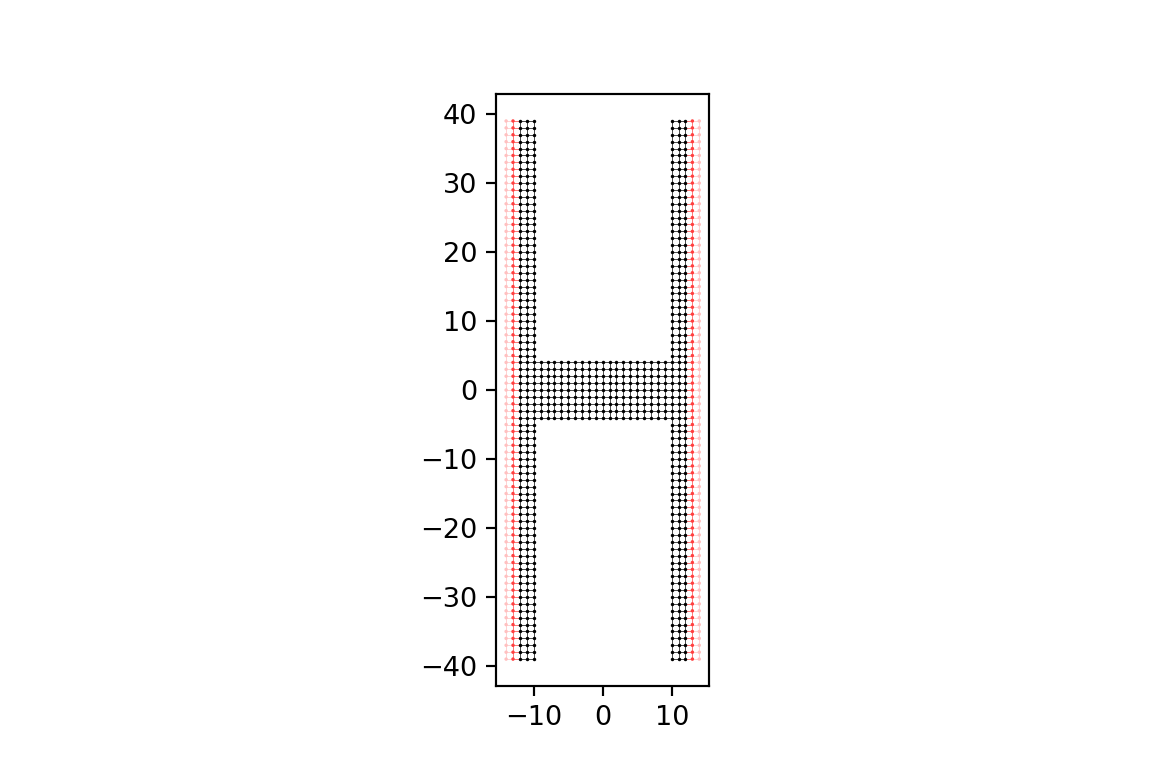
\includegraphics[width=0.45\textwidth]{./media/2degconst_W5_L10.png}
  \caption{Plot of a square lattice quantum point contact of width $W=5$ and
  length $L=10$ defined in kwant.}
  \label{fig:2degconst_W5_L10}
  \end{center}
\end{figure}

The quantum point contacts have a specific, quantized conductance in function of energy \cite{QPCarticle}.
I calculated the transmission coefficients of the structure shown in figure \ref{fig:2degconst_W5_L10},
and plotted against the energy. The results (shown in fig. \ref{fig:cond_2deg_W5_L10_VL6_0_VS6_0.png}.)
reflect the transmission quantization presented in \cite{QPCarticle}.
\begin{figure}[H]
  \begin{center}
  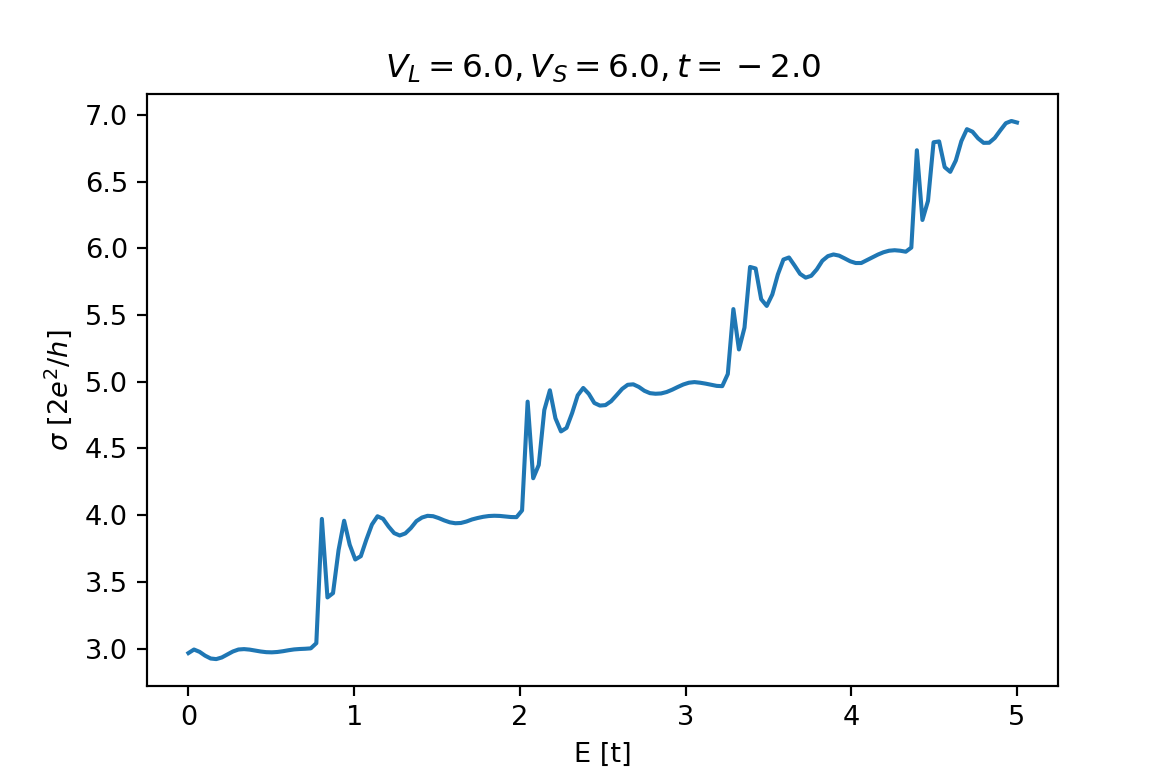
\includegraphics[width=0.45\textwidth]{./media/cond_2deg_W5_L10_VL6_0_VS6_0.png}
  \caption{Transmission coefficients calculated using the system shown in figure \ref{fig:2degconst_W5_L10}.
  The potential in the scattering region and in leads is $V_L=V_S=6\textrm{eV}$, while the
  hopping energy is $t=-2\textrm{eV}$.}
  \label{fig:cond_2deg_W5_L10_VL6_0_VS6_0.png}
  \end{center}
\end{figure}

Using kwants built-in function \texttt{kwant.physics.two\_terminal\_shotnoise},
I was able to easily calculate the shot-noise \cite{shotnoise} between leads. 
I created the structure shown on figure \ref{fig:2degconst_W5_L10}, then calculated
the two-terminal shot-noise between leads. The results are shown on figure \ref{fig:shotnoise_2deg_W5_L10_VL6_0_VS6_0}.
\begin{figure}[H]
  \begin{center}
  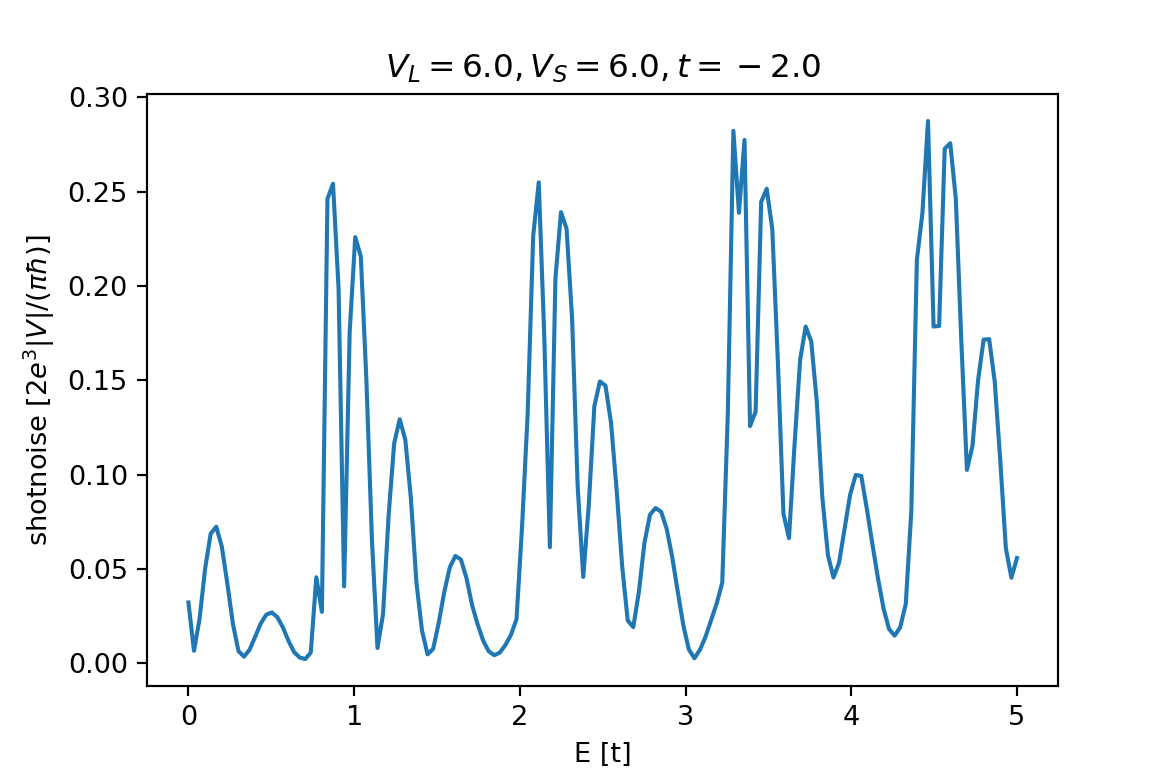
\includegraphics[width=0.45\textwidth]{./media/shotnoise_2deg_W5_L10_VL6_0_VS6_0.png}
  \caption{Shot noise in function of the electron energy.}
  \label{fig:shotnoise_2deg_W5_L10_VL6_0_VS6_0}
  \end{center}
\end{figure}
If a tight-binding system is placed in magnetic field, this can be taken into account by using Peierls' substitution:
\begin{equation*}
  t_{ij} \rightarrow t_{ij} \times \exp\left(i \frac{e}{\hbar} \int_{\mathbf{x}_j}^{\mathbf{x}_i} \mathbf{A}(\mathbf{x}) d\mathbf{s}\right)
\end{equation*}

For 2D square lattices this can be rewritten as 
\begin{equation*}
  \exp\left(i\, 2 \pi \frac{\phi}{\phi_0} \frac{(y_i + y_j)(x_i-x_j)}{2a^2} \right)  
\end{equation*}
where $\phi = B a^2$ is the flux through a unit cell in the square lattice,
and $\phi_0 = h/e$ is the magnetic flux quantum. To study the effect of magnetic field in case of 
2D square lattices, I defined a quantum point contact in kwant. This structure is shown on figure
\ref{fig:qpc_L15_W5}.

\begin{figure}[H]
  \begin{center}
  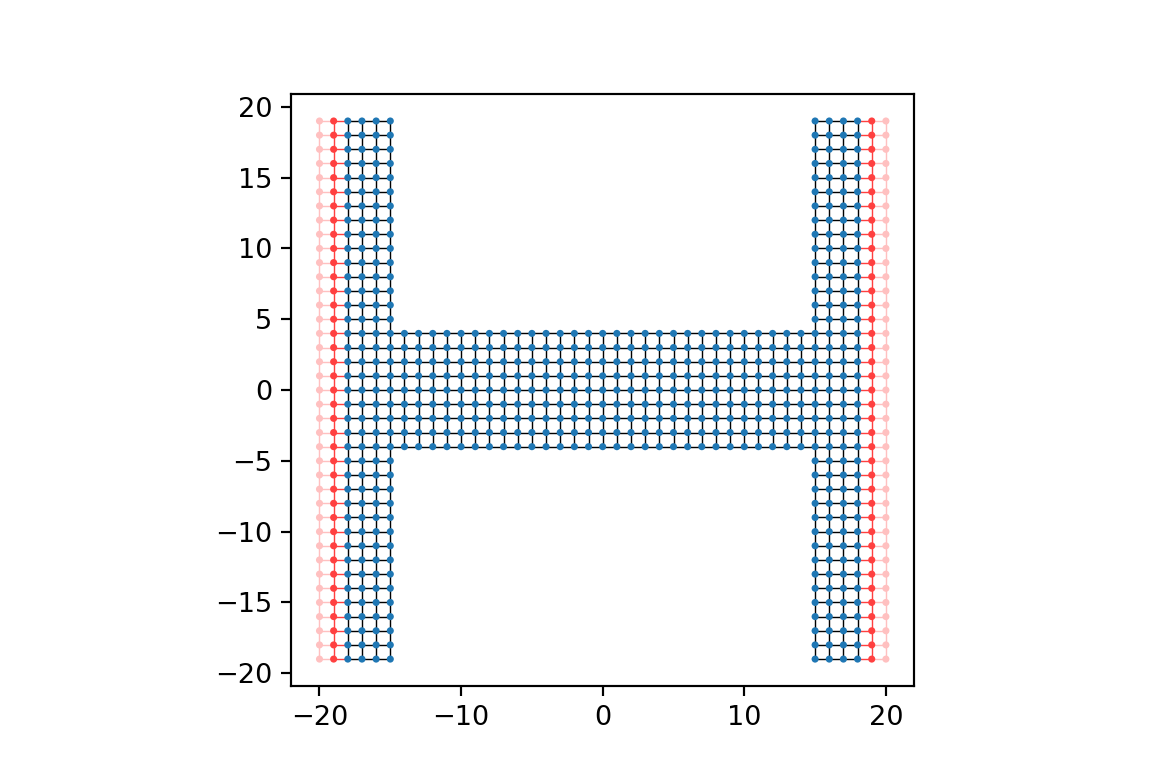
\includegraphics[width=0.45\textwidth]{./media/qpc_L15_W5.png}
  \caption{A quantum point contact of width $W=5$ and length $L=15$ defined and plotted using kwant.}
  \label{fig:qpc_L15_W5}
  \end{center}
\end{figure}

Using kwant's built-in functions, I calculated the transmission coefficients between leads $0$
and $1$, for a range of magnetic field strengths. Th results are plotted on figure \ref{fig:qpc_L15_W5_VS0_2_cond_phi_e1_5}.

\begin{figure}[H]
  \begin{center}
  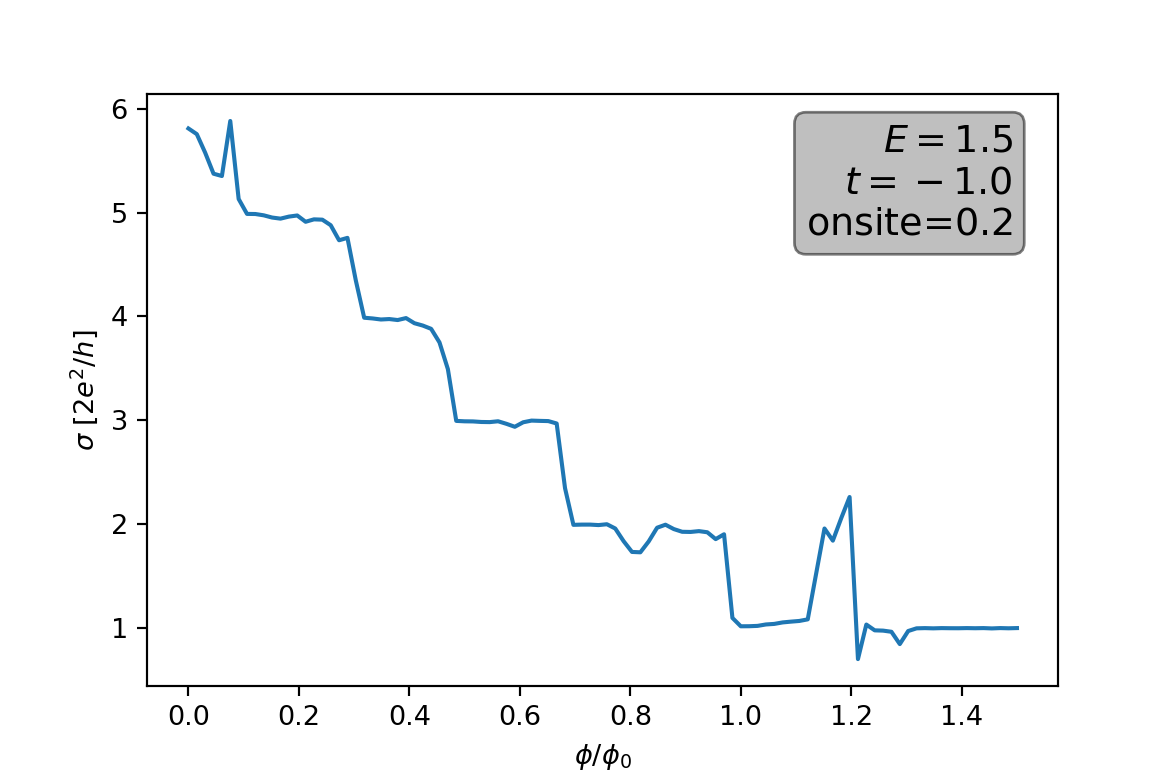
\includegraphics[width=0.45\textwidth]{./media/qpc_L15_W5_VS0_2_cond_phi_e1_5.png}
  \caption{Transmission coefficient of a quantum point contact as a function of the external magnetic flux.}
  \label{fig:qpc_L15_W5_VS0_2_cond_phi_e1_5}
  \end{center}
\end{figure}

\section*{Graphene minimal conductivity}


\section*{topological Anderson Insulators}
\begin{equation*}
  \mathcal H = \sum\limits_i V_{\textrm{dis}}\ket i \bra i + \sum\limits_{<i,j>} t_{ij} \ket i \bra j
\end{equation*}
\begin{equation*}
  V_\text{dis} = \sum_i W_i \ket i \bra i
\end{equation*}
\begin{equation*}
  t_{ij} = \exp\left(i\, 2 \pi \frac{\phi}{\phi_0} \frac{(y_i + y_j)(x_i-x_j)}{2a^2} \right)
\end{equation*}

\begin{figure}[H]
  \begin{center}
  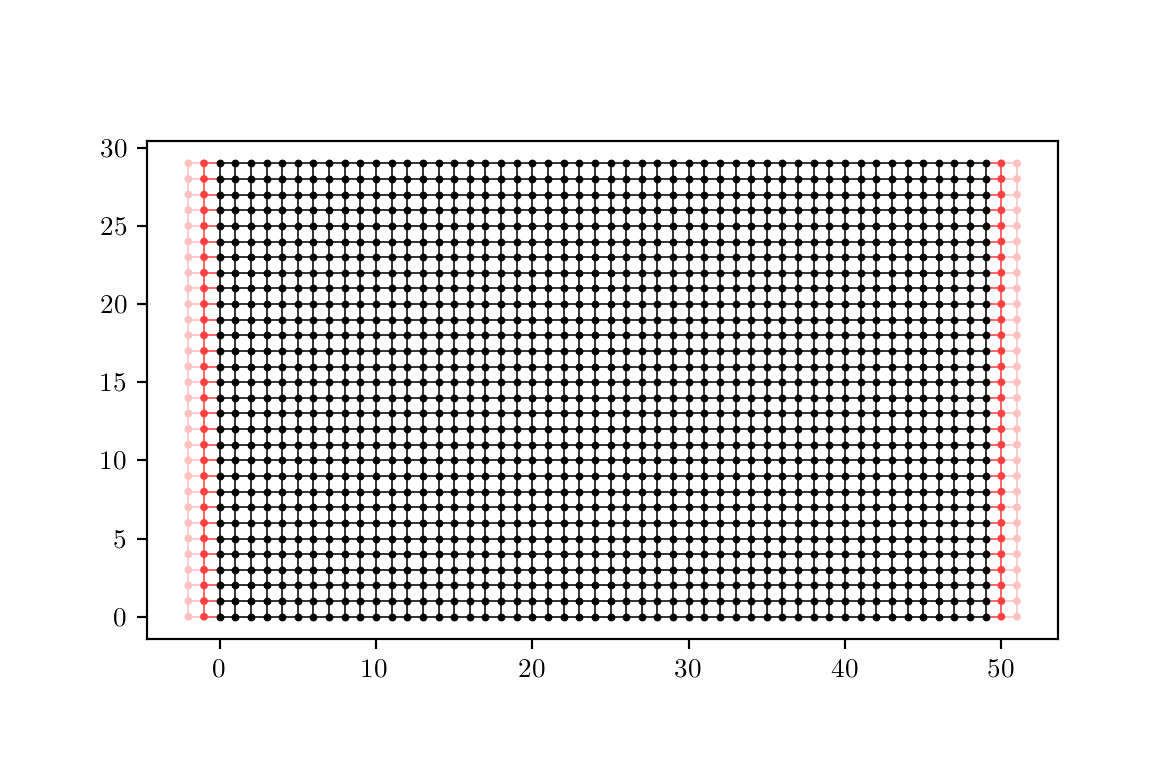
\includegraphics[width=0.45\textwidth]{./media/square_lattice_W=30_L=50.png}
  \caption{}
  \label{fig:square_lattice_W_30_L_50}
  \end{center}
\end{figure}

\begin{figure}[H]
  \begin{center}
  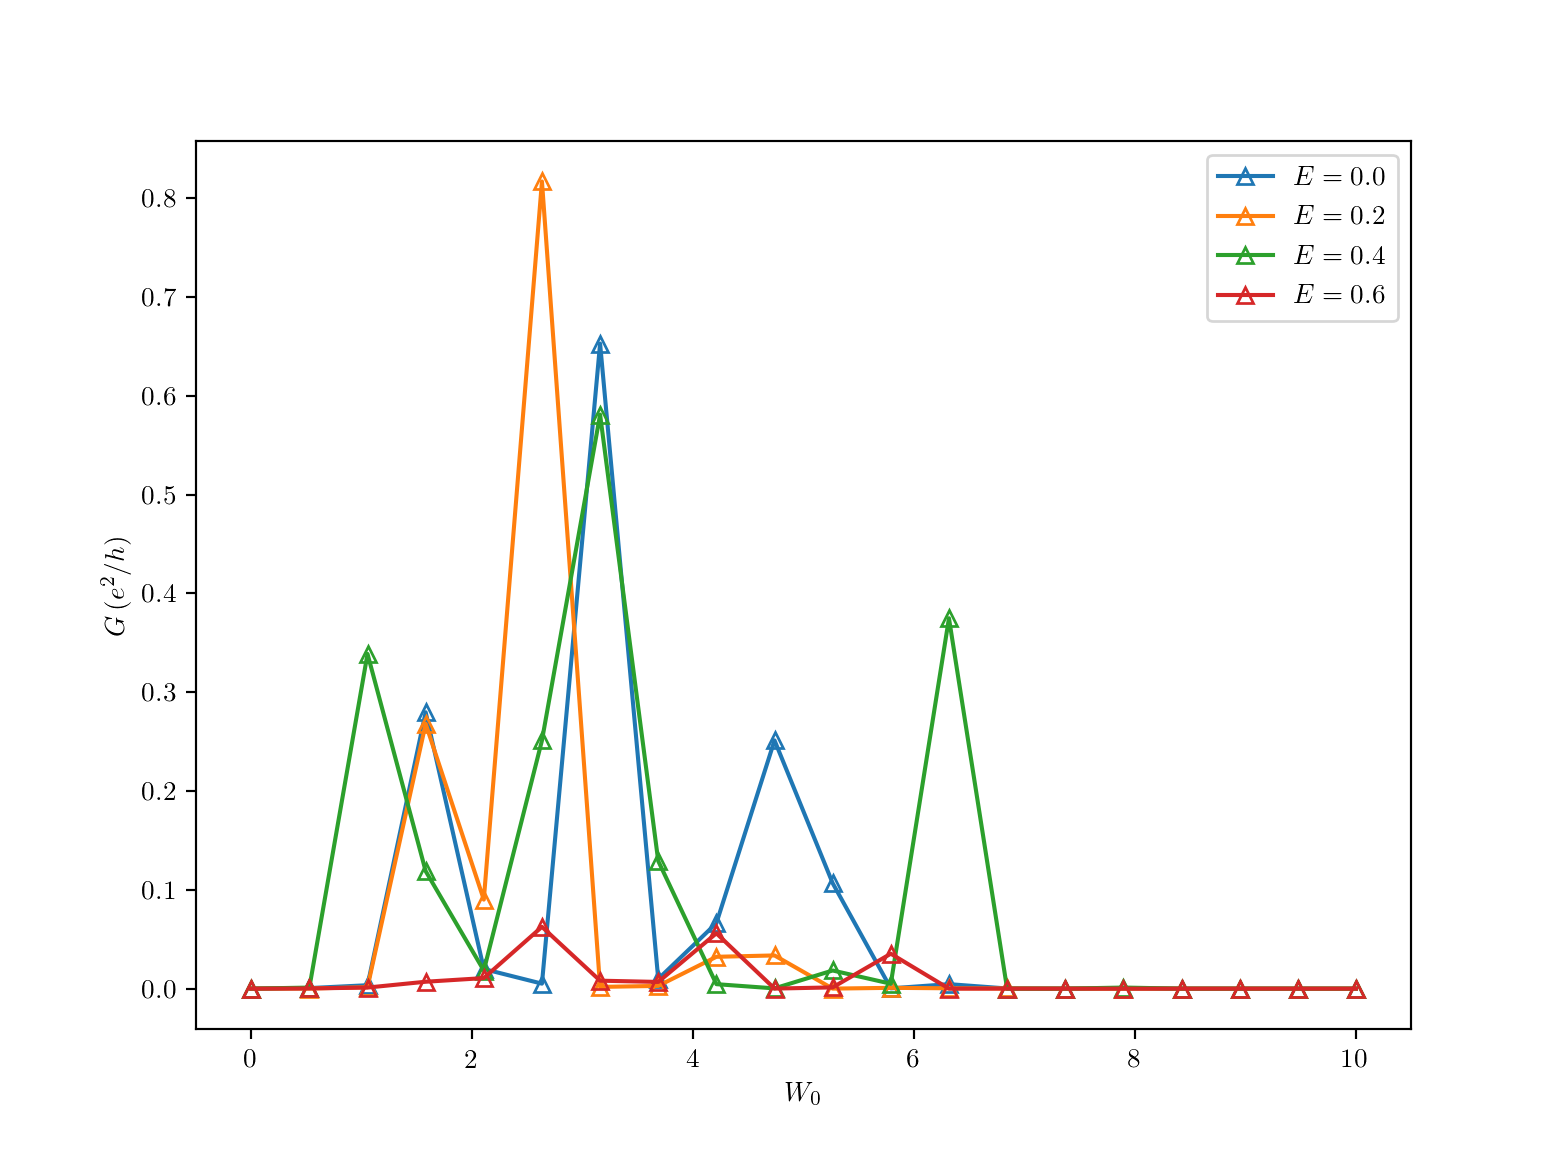
\includegraphics[width=0.45\textwidth]{./media/transmission_square_lat_phi=0dot0.png}
  \caption{}
  \label{fig:transmission_square_lat_phi_0dot0}
  \end{center}
\end{figure}

\begin{figure}[H]
  \begin{center}
  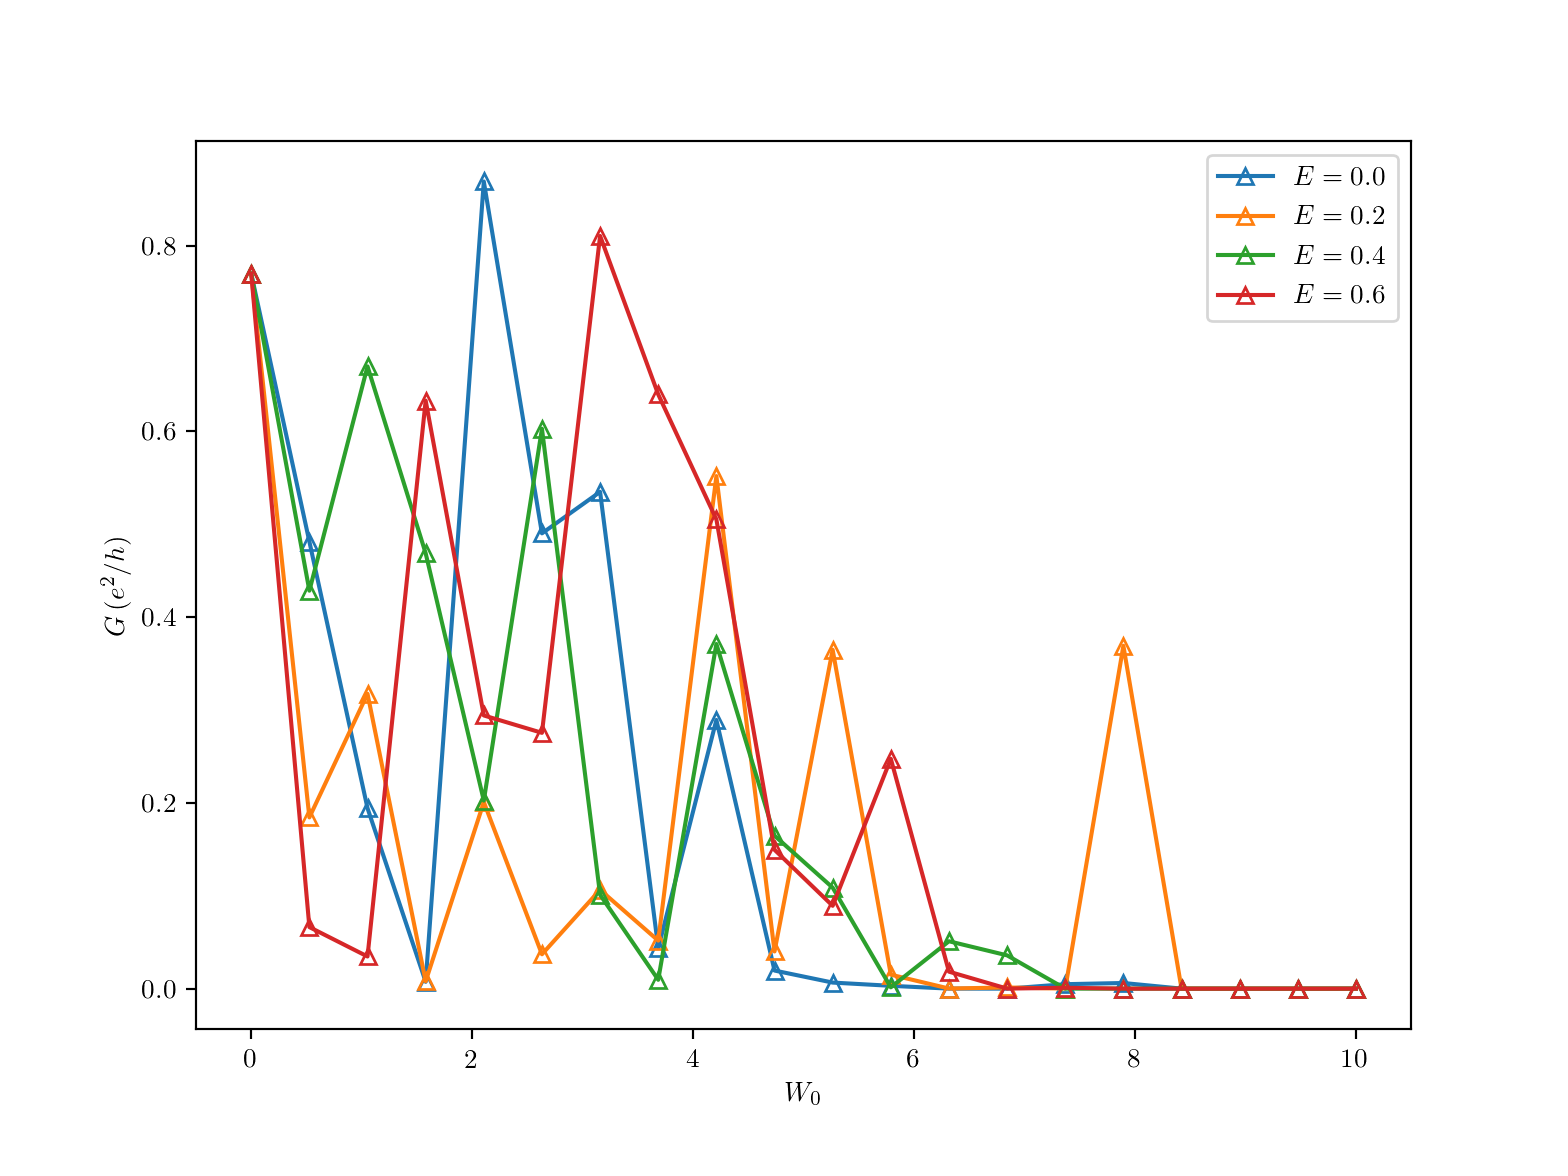
\includegraphics[width=0.45\textwidth]{./media/transmission_square_lat_phi=0dot2.png}
  \caption{}
  \label{fig:transmission_square_lat_phi_0dot2.png}
  \end{center}
\end{figure}

\begin{figure}[H]
  \begin{center}
  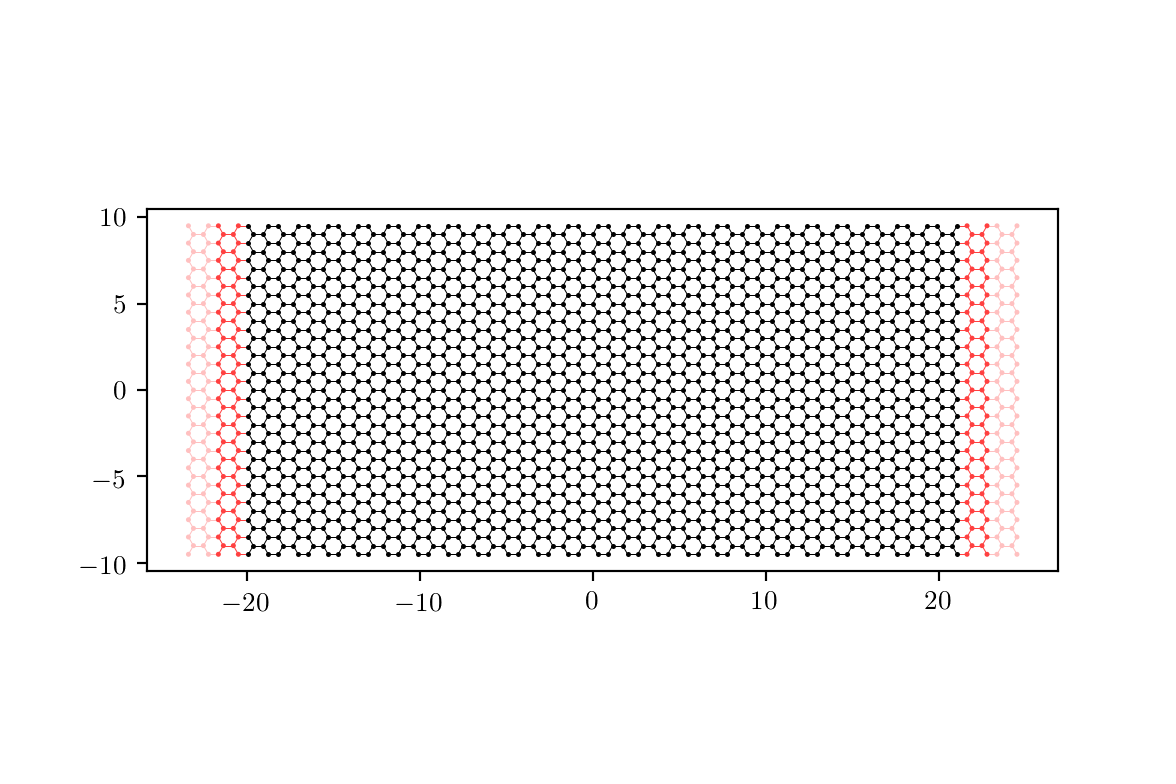
\includegraphics[width=0.45\textwidth]{./media/graphene_lattice_W=20_L=40.png}
  \caption{}
  \label{fig:graphene_lattice_W_20_L_40.png}
  \end{center}
\end{figure}

\begin{figure}[H]
  \begin{center}
  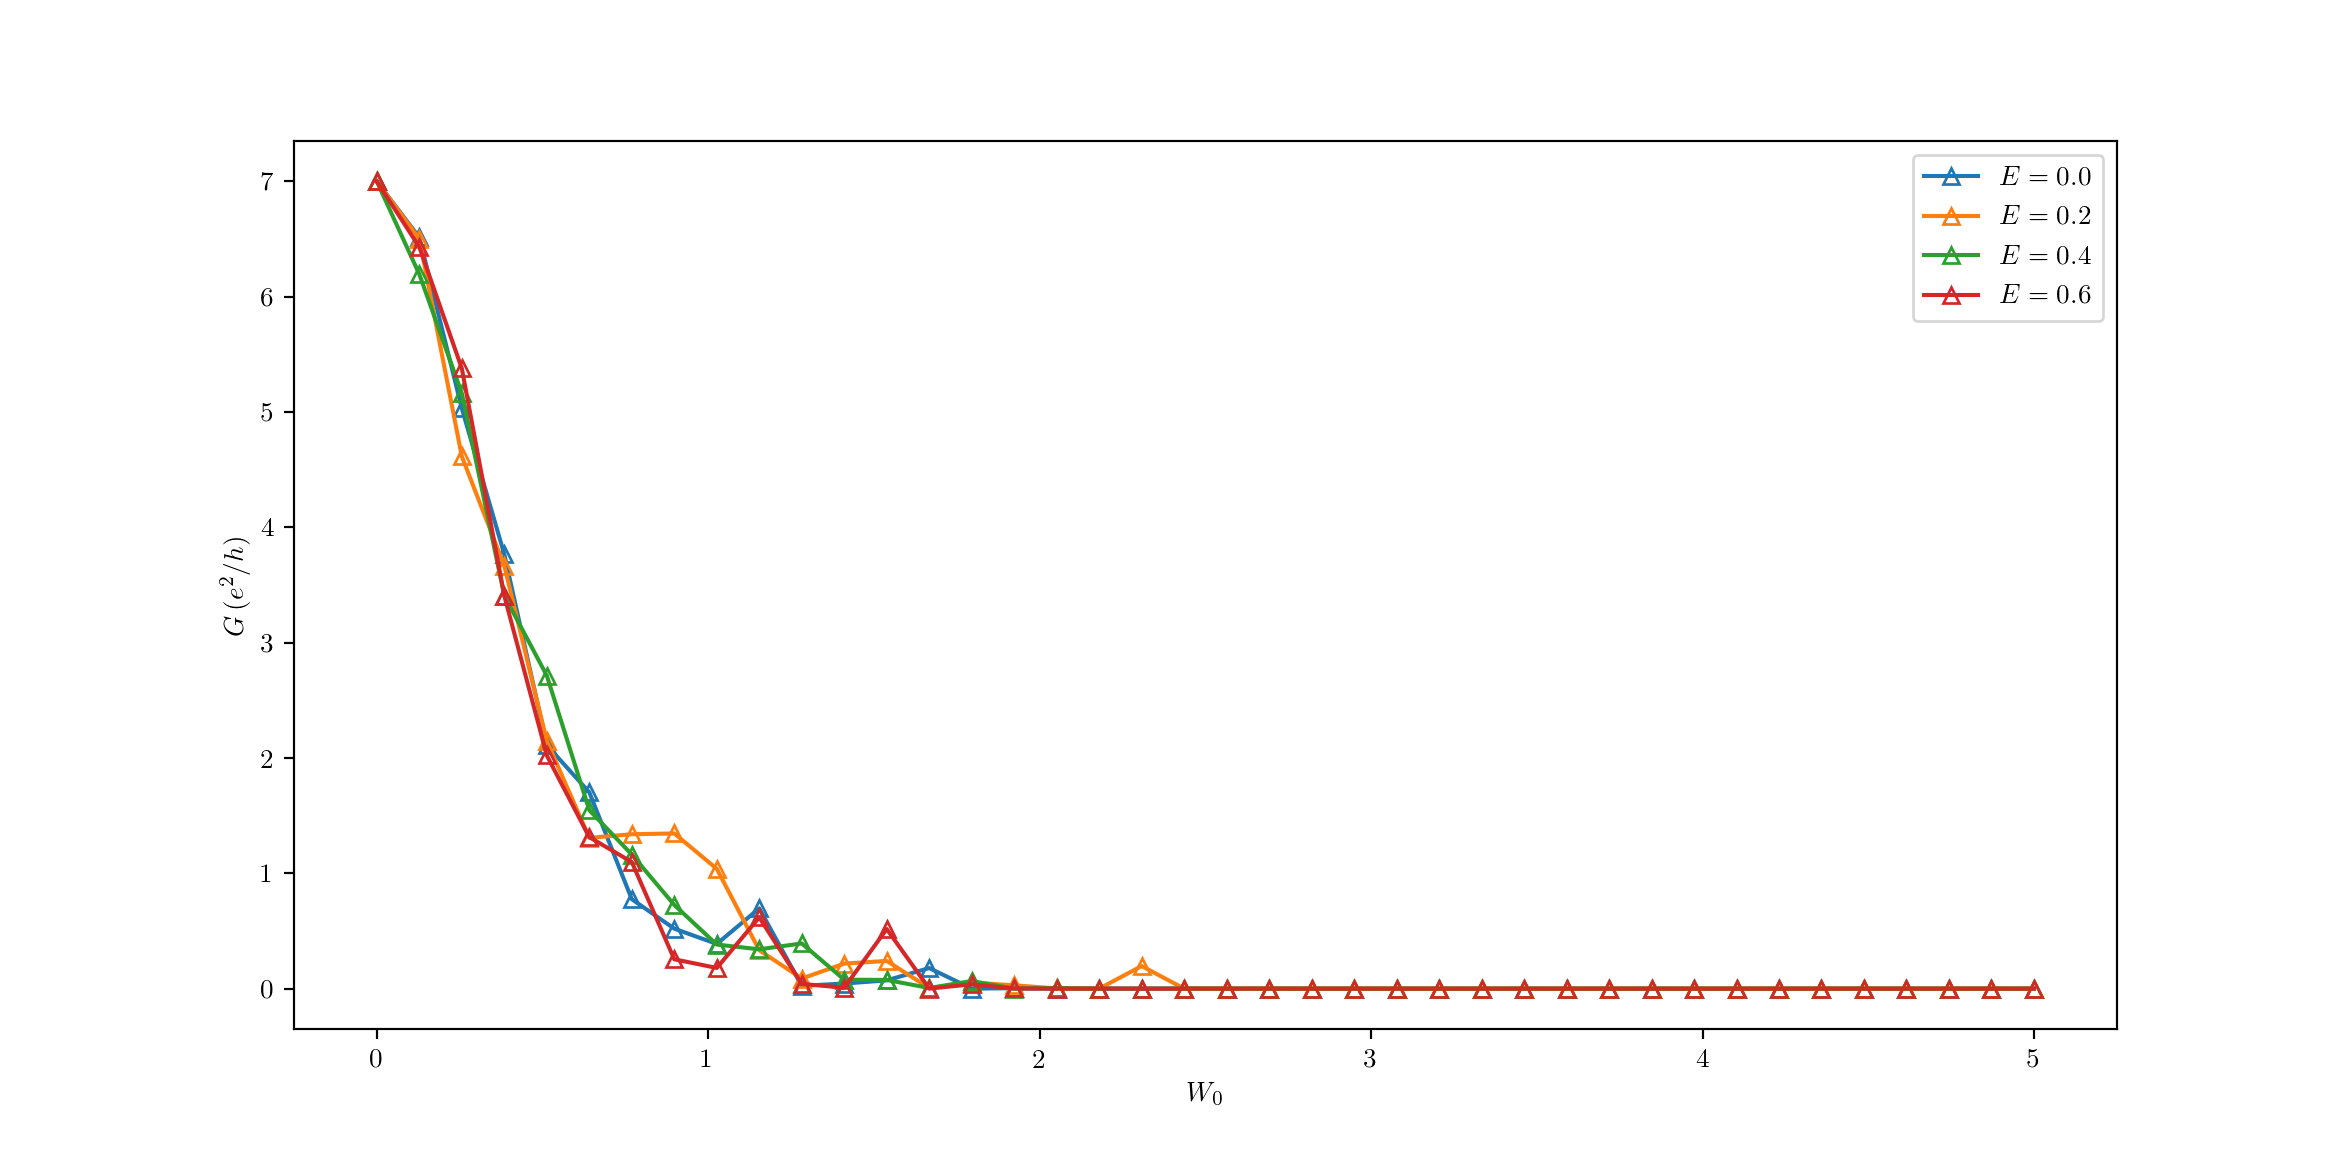
\includegraphics[width=0.45\textwidth]{./media/transmission_graphene_lat_phi=0dot0Wmax=5.png}
  \caption{}
  \label{fig:transmission_graphene_lat_phi_0dot0Wmax_5.png}
  \end{center}
\end{figure}

\begin{figure}[H]
  \begin{center}
  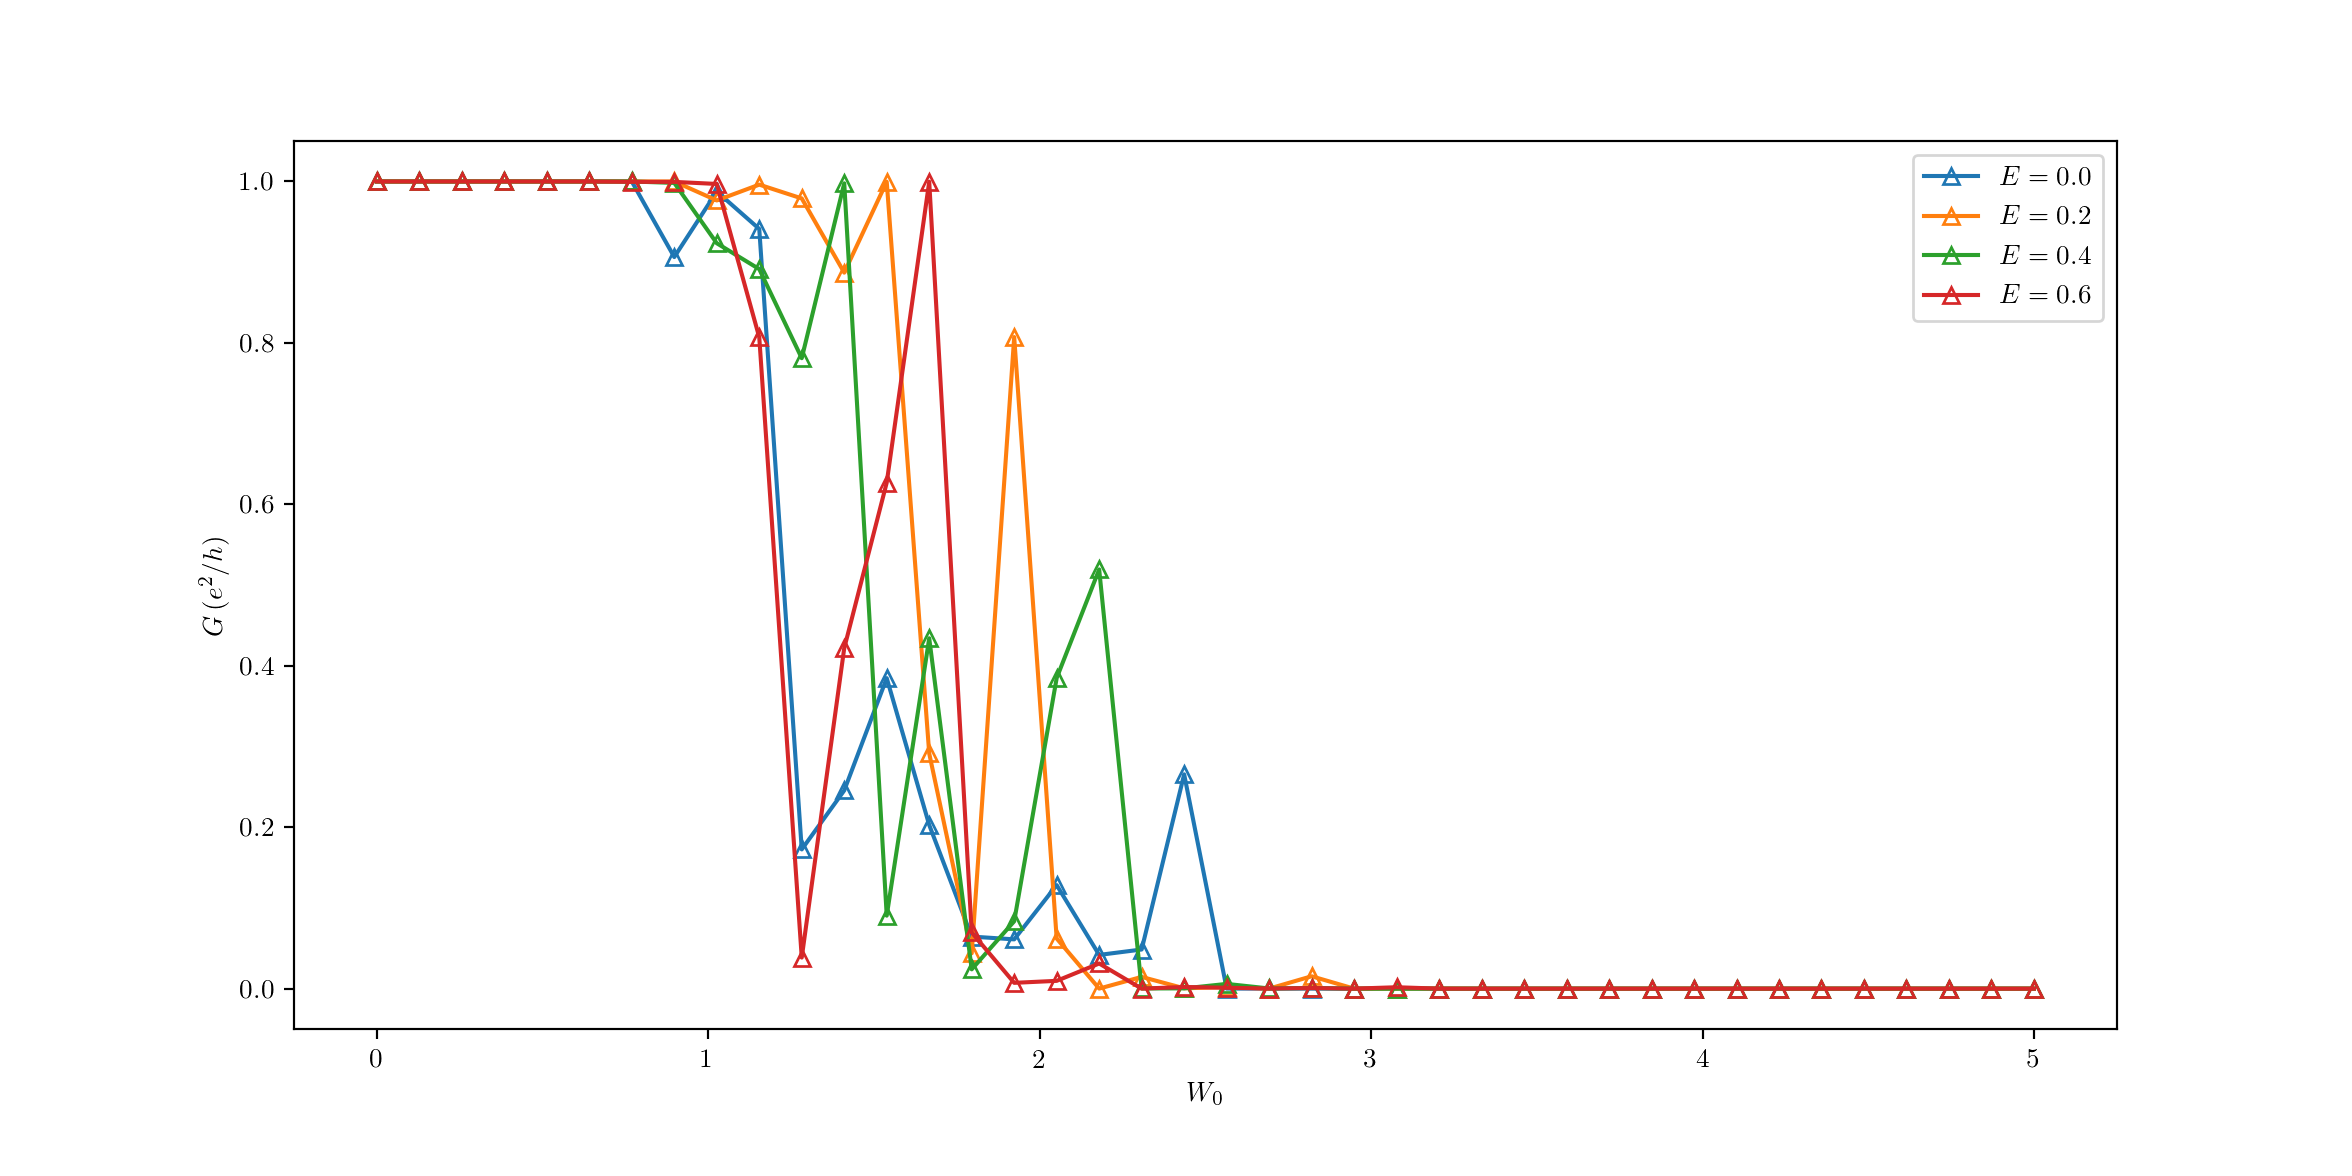
\includegraphics[width=0.45\textwidth]{./media/transmission_graphene_lat_phi=0dot6Wmax=5.png}
  \caption{}
  \label{fig:transmission_graphene_lat_phi_0dot6Wmax_5.png}
  \end{center}
\end{figure}

%%%%%%%%%%%%%%
% References %
%%%%%%%%%%%%%%

\nocite{*}
\bibliographystyle{plain}
\bibliography{references}

%%%%%%%%%%%%%%
% Appendices %
%%%%%%%%%%%%%%
\appendix
\section{Some appendix}
\subsection{Some subsection}


\end{document}

